\documentclass[12pt,fleqn]{article}\usepackage{../common}
\begin{document}
Paralel KMeans, Hadoop

K-Means algoritmasini nasil paralel sekilde isletiriz? Ozellikle Hadoop gibi bir Esle-Indirge (Map-Reduce) ortamini dusunelim. Veri cok buyuk olcekte olabilir ve bu veriler birden fazla makinaya bolunecektir. Esle-Indirge kavraminda esleme safhasinda "anahtar uretiriz", ve sonra indirgeme safhasinda Hadoop sistemi oyle kurmustur
ki ayni anahtarlarlar tek bir makinaya gonderilir, ve bu nihai asamada artik anahtar bazinda indirgeme (ozetleme) yapilir.

Paralel K-Means icin anahtar nedir? Anahtar, mesela kume olabilir. Yani kume 1, kume 2 gibi kume
isaretleri / sayilari anahtar olarak kullanilabilirler.

Peki anahtar ile eslenecek "deger" nedir?

Oyle bir deger ariyoruz ki ust uste konulabilecek bir sey olmali, EI sisteminin kuvveti burada, anahtarlar farkli noktalarda
uretilebiliyor, sonra tek noktada ust uste konuyor, o zaman degerler oyle uretilmeli ki bu ust uste koyma, ozetleme islemi yapilabilsin.

Ust uste konabilecek sey kumeye (anahtar) ait olan veri noktasi olabilir, yani basbasyagi veri noktasinin kendisi deger olabilir.  Normal K-Means'i hatirlarsak, her nokta icin o noktaya en yakin kumeyi buluyordu ve sonra, atama islemi bitince, her kumenin altindaki noktalarin toparlayip, onlarin ortalamasini alarak yeni kume merkezini hesapliyordu. Bu ortalama islemi ust uste konabilecek bir sey, cunku toplama oyle bir islem, ve / yani farkli makinalarda kume-nokta, eslemelerini uretirsek, indirgeme asamasinda o anahtar icin tum degerleri toplayip, nokta sayisina boleriz ve yeni kume merkezini elde ederiz. 

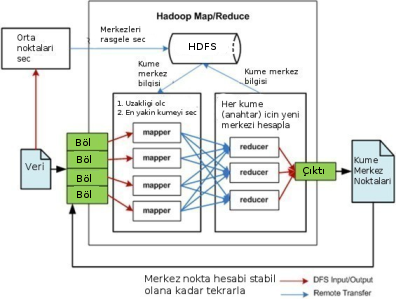
\includegraphics[height=8cm]{kmeans-diag.png}

Simdi Hadoop ile ilgili bazi lojistik konulara gelelim:

Eger esleme safhasinda her nokta icin en yakin kumeyi bulmak
istiyorsak, o zaman (ilk basta rasgele bile olsa) kume merkezlerinin
bilgisi tum makinalarin erisebilecegi bir yerde olmali. Biz bu veriyi,
\verb!centers.csv! adli bir dosyaya koymaya karar verdik, bu dosya
tek makina ortaminda bilinen bir dizinde (mesela /tmp), cok makinali ortamda
ise HDFS uzerinde herkesin erisebilecegi bir yerde olmali. 

Paralel K-Means icin tek bir esle-indirge isletimi yeterli degil, bu
algoritma dongulu / ozyineli (iterative) bir algoritma, 5,10,20 kez
islemesi gerekebilir.  Her dongu (indirgeme) sonunda yeni kume
merkezleri hesaplanacak, bu merkezler eski \verb!centers.csv!
yerini alacak ve islem tekrar baslayacak.

Simdi ham veriyi gosterelim,

\begin{minted}{python}
from pandas import *
df1 = read_csv("synthetic.txt",sep="   ")
plt.scatter(df1.ix[:,0],df1.ix[:,1])
plt.savefig('kmeans_1.png')
\end{minted}

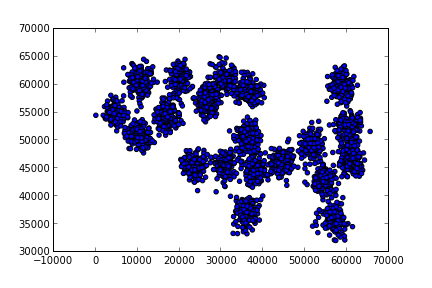
\includegraphics[height=4cm]{kmeans_1.png}

\inputminted{python}{kmeans.py}

\verb!reduce_all_centers! cagrisi tum indirgeyiciler her kume icin yeni
orta noktayi hesaplayip onu yayinladiktan (emit) sonra, tum yeni
merkezlerin gelecegi yer.

Komut satirindan tek makina icin Hadoop'suz isletelim,

\begin{minted}{python}
!sort --random-sort synthetic.txt > /tmp/synthetic.txt
!head -15 /tmp/synthetic.txt > /tmp/centers.csv
!python kmeans.py synthetic.txt
\end{minted}

\begin{verbatim}
/usr/local/lib/python2.7/dist-packages/pytz/__init__.py:29: UserWarning: Module _yaml was already imported from /usr/lib/python2.7/dist-packages/_yaml.so, but /usr/local/lib/python2.7/dist-packages is being added to sys.path
  from pkg_resources import resource_stream
using configs in /home/burak/.mrjob.conf
creating tmp directory /tmp/kmeans.burak.20131202.234454.312709
writing to /tmp/kmeans.burak.20131202.234454.312709/step-0-mapper_part-00000
Counters from step 1:
  (no counters found)
writing to /tmp/kmeans.burak.20131202.234454.312709/step-0-mapper-sorted
> sort /tmp/kmeans.burak.20131202.234454.312709/step-0-mapper_part-00000
writing to /tmp/kmeans.burak.20131202.234454.312709/step-0-reducer_part-00000
Counters from step 1:
  (no counters found)
writing to /tmp/kmeans.burak.20131202.234454.312709/step-1-mapper_part-00000
Counters from step 2:
  (no counters found)
writing to /tmp/kmeans.burak.20131202.234454.312709/step-1-mapper-sorted
> sort /tmp/kmeans.burak.20131202.234454.312709/step-1-mapper_part-00000
writing to /tmp/kmeans.burak.20131202.234454.312709/step-1-reducer_part-00000
10 [ 33655.97916667  59869.70138889]
13 [ 10318.87456446  55430.98780488]
9 [ 21286.26027397  59328.61187215]
0 [ 34297.27789474  43563.19789474]
1 [ 56490.3362069   37260.18103448]
2 [ 56217.97297297  43823.02702703]
3 [ 56453.07407407  34324.16666667]
4 [ 22960.27741935  45942.7483871 ]
5 [ 61346.1443299   47761.37113402]
6 [ 58466.11940299  60120.6641791 ]
7 [ 51691.66477273  48608.63636364]
8 [ 60189.47019868  53209.15231788]
11 [ 62427.68  44841.88]
12 [ 27699.59813084  56743.19626168]
14 [ 41850.40925267  47055.58362989]
Counters from step 2:
  (no counters found)
Moving /tmp/kmeans.burak.20131202.234454.312709/step-1-reducer_part-00000 -> /tmp/kmeans.burak.20131202.234454.312709/output/part-00000
Streaming final output from /tmp/kmeans.burak.20131202.234454.312709/output
removing tmp directory /tmp/kmeans.burak.20131202.234454.312709
using configs in /home/burak/.mrjob.conf
using configs in /home/burak/.mrjob.conf
creating tmp directory /tmp/kmeans.burak.20131202.234456.597838
creating tmp directory /tmp/kmeans.burak.20131202.234456.597838
writing to /tmp/kmeans.burak.20131202.234456.597838/step-0-mapper_part-00000
writing to /tmp/kmeans.burak.20131202.234456.597838/step-0-mapper_part-00000
Counters from step 1:
Counters from step 1:
  (no counters found)
  (no counters found)
writing to /tmp/kmeans.burak.20131202.234456.597838/step-0-mapper-sorted
writing to /tmp/kmeans.burak.20131202.234456.597838/step-0-mapper-sorted
> sort /tmp/kmeans.burak.20131202.234456.597838/step-0-mapper_part-00000
> sort /tmp/kmeans.burak.20131202.234456.597838/step-0-mapper_part-00000
writing to /tmp/kmeans.burak.20131202.234456.597838/step-0-reducer_part-00000
writing to /tmp/kmeans.burak.20131202.234456.597838/step-0-reducer_part-00000
Counters from step 1:
Counters from step 1:
  (no counters found)
  (no counters found)
writing to /tmp/kmeans.burak.20131202.234456.597838/step-1-mapper_part-00000
writing to /tmp/kmeans.burak.20131202.234456.597838/step-1-mapper_part-00000
Counters from step 2:
Counters from step 2:
  (no counters found)
  (no counters found)
writing to /tmp/kmeans.burak.20131202.234456.597838/step-1-mapper-sorted
writing to /tmp/kmeans.burak.20131202.234456.597838/step-1-mapper-sorted
> sort /tmp/kmeans.burak.20131202.234456.597838/step-1-mapper_part-00000
> sort /tmp/kmeans.burak.20131202.234456.597838/step-1-mapper_part-00000
writing to /tmp/kmeans.burak.20131202.234456.597838/step-1-reducer_part-00000
writing to /tmp/kmeans.burak.20131202.234456.597838/step-1-reducer_part-00000
10 [ 34190.76071429  59473.68214286]
13 [  9524.38372093  55188.34689922]
9 [ 19288.00425532  59048.12340426]
0 [ 34495.96781609  42837.15862069]
1 [ 56603.56756757  37301.28378378]
2 [ 54698.1862069   43080.47586207]
3 [ 56850.95180723  34689.86746988]
4 [ 23627.50314465  45589.86792453]
5 [ 60775.48039216  47705.81372549]
6 [ 58623.54054054  59894.10135135]
7 [ 51384.90184049  49124.60736196]
8 [ 60238.23021583  52723.48920863]
11 [ 61762.52830189  45110.81132075]
12 [ 27191.86813187  57337.64835165]
14 [ 41387.76223776  47391.7972028 ]
...
\end{verbatim}

\begin{minted}{python}
import pandas as pd
df1 = pd.read_csv("synthetic.txt",sep="   ",header=None)
plt.scatter(df1.ix[:,0],df1.ix[:,1])
plt.hold(True)
df2 = pd.read_csv("/tmp/centers.csv", sep="   ", header=None)
plt.plot(df2.ix[:,0],df2.ix[:,1],'rd')
plt.savefig('kmeans_2.png')
\end{minted}

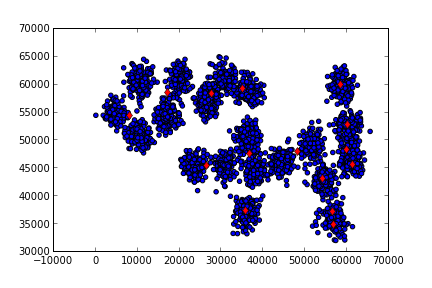
\includegraphics[height=4cm]{kmeans_2.png}

K-Means'i 20 kere islettik. Eger istenirse (hatta daha iyi olur) dongu bir
\verb!while! icine konur ve bitis icin "stabilite sarti"
aranir. Stabilite yeni kume merkezinin eskisinden "cok fazla degisik olup
olmadigi" sartidir, degisim yoksa artik sonucu bulmusuz demektir, daha
fazla donguye gerek kalmayacaktir. Biz donguyu 20 kere donguyu islettik,
(bu problem icin) yeterli oldu.

K-Means isini bitirdikten sonra elde edilen sonuclari okuyabiliriz. Nihai
kume merkezleri \verb!/tmp/centers.csv! icinde. Bu merkezleri alip,
ham veri uzerinde kirmizi nokta olarak gosteriyoruz.

veriyi 20-30 makinaya dagitarak parca parca isleyip kumelemeniz
mumkundur. Endustride son zamanlarda habire duyulan Buyuk Veri (Big Data)
olayi iste bu.



\end{document}
